%En el grafico se puede observar como el crecimiento de todos las heuristicas es polinomial a menida que el grafo aumenta su densidad en aristas. A su vez el algoritmo $Tabu$ $Search$ presenta una mayor diferencia en cuanto a tiempo, esto es razonable porque puede empeorar parcialmente la solucion dependiendo la cantidad de nodos, entonces esa diferencia (constante) lo que hace es "subirme" la funcion la cantidad observada. 

Para realizar la experimentación respecto a la calidad de las heurísticas presentadas, utilizamos un generador de los siguientes grafos:
\begin{itemize}
\item Estrella + CMF
\item Estrella+Puente+CMF
\item Estrella+Puente+Doble Estrella
\item Banana Tree (Palmera)
\item Rueda
\end{itemize}

 \begin{figure}[H] %[h] Aqui [b] para button [t] para top
\begin{center}
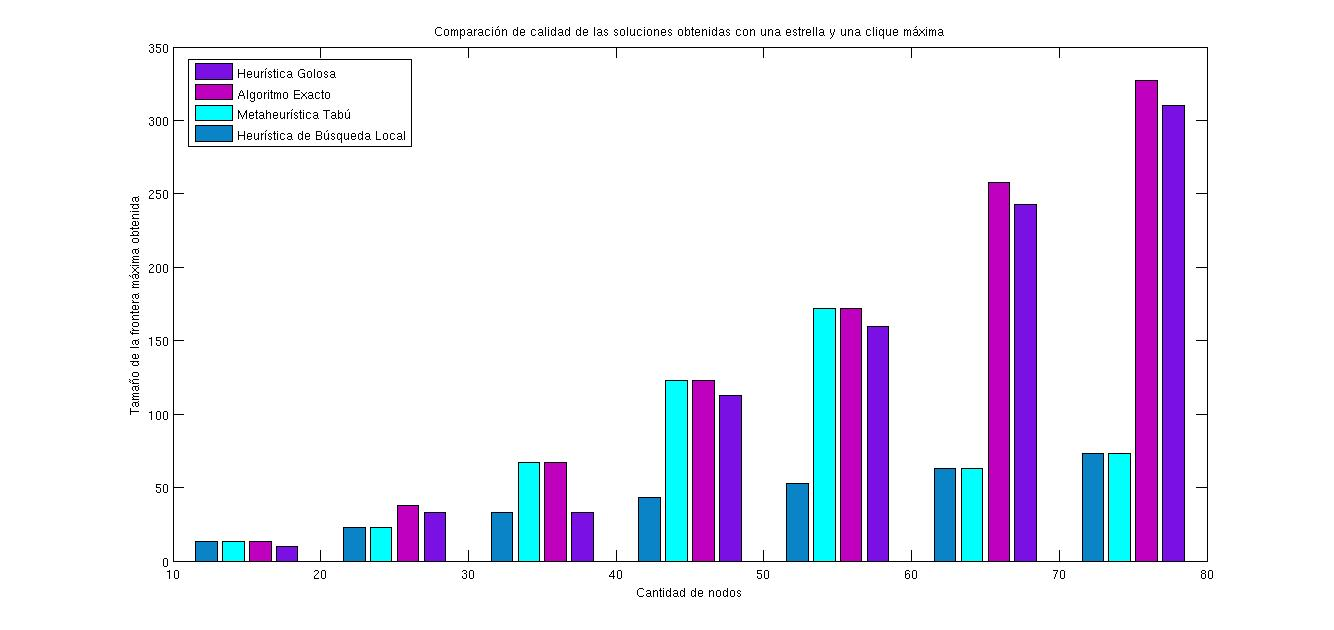
\includegraphics[width=400pt]{../imgs/calidadSolucionesChicas15.jpg}
\caption{Comparación realizada con soluciones chicas con un grafo de tipo Estrella+CMF.}
\end{center}
\end{figure}

 \begin{figure}[H] %[h] Aqui [b] para button [t] para top
\begin{center}
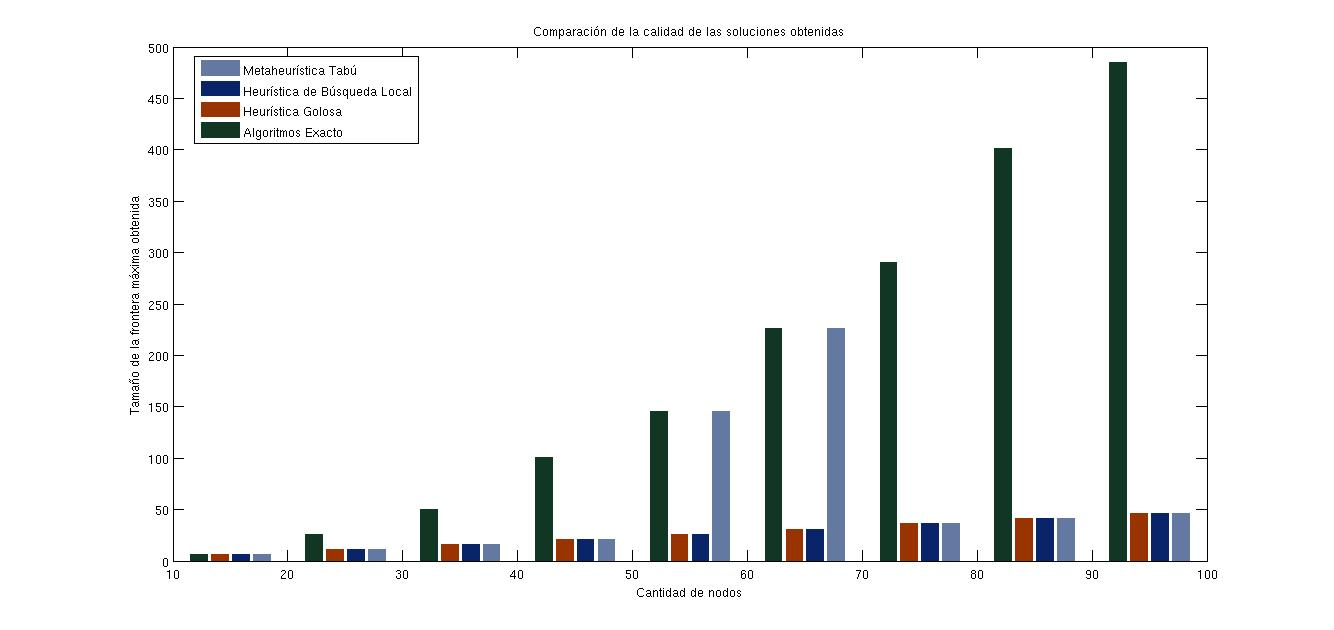
\includegraphics[width=400pt]{../imgs/calidadSolucionesChica14.jpg}
\caption{Comparación realizada con soluciones chicas con un grafo de tipo Estrella+Puente+CMF.}
\end{center}
\end{figure}

 \begin{figure}[H] %[h] Aqui [b] para button [t] para top
\begin{center}
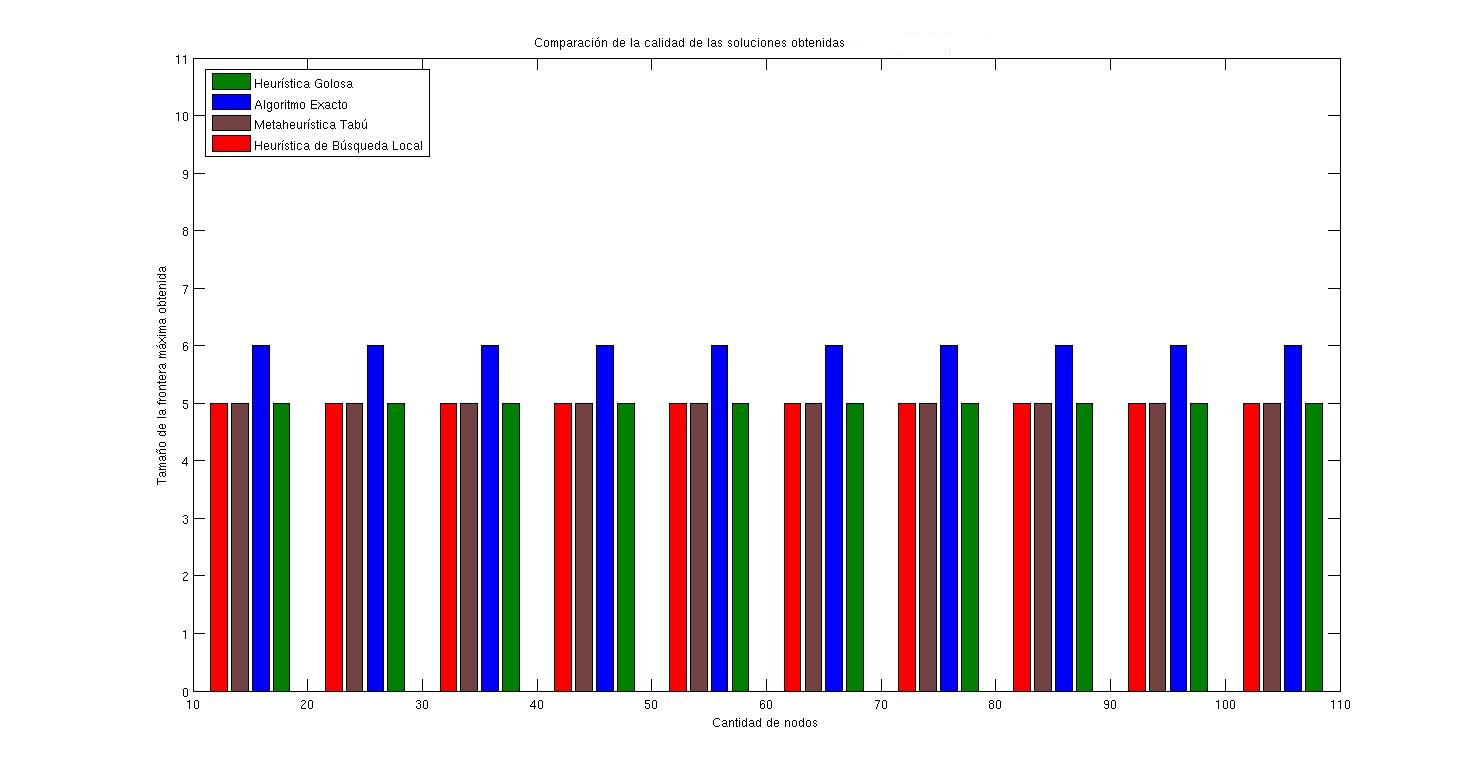
\includegraphics[width=400pt]{../imgs/calidadSolucionesChicas17.jpg}
\caption{Comparación realizada con soluciones chicas con un grafo de tipo Estrella+Puente+Doble Estrella.}
\end{center}
\end{figure}

 \begin{figure}[H] %[h] Aqui [b] para button [t] para top
\begin{center}
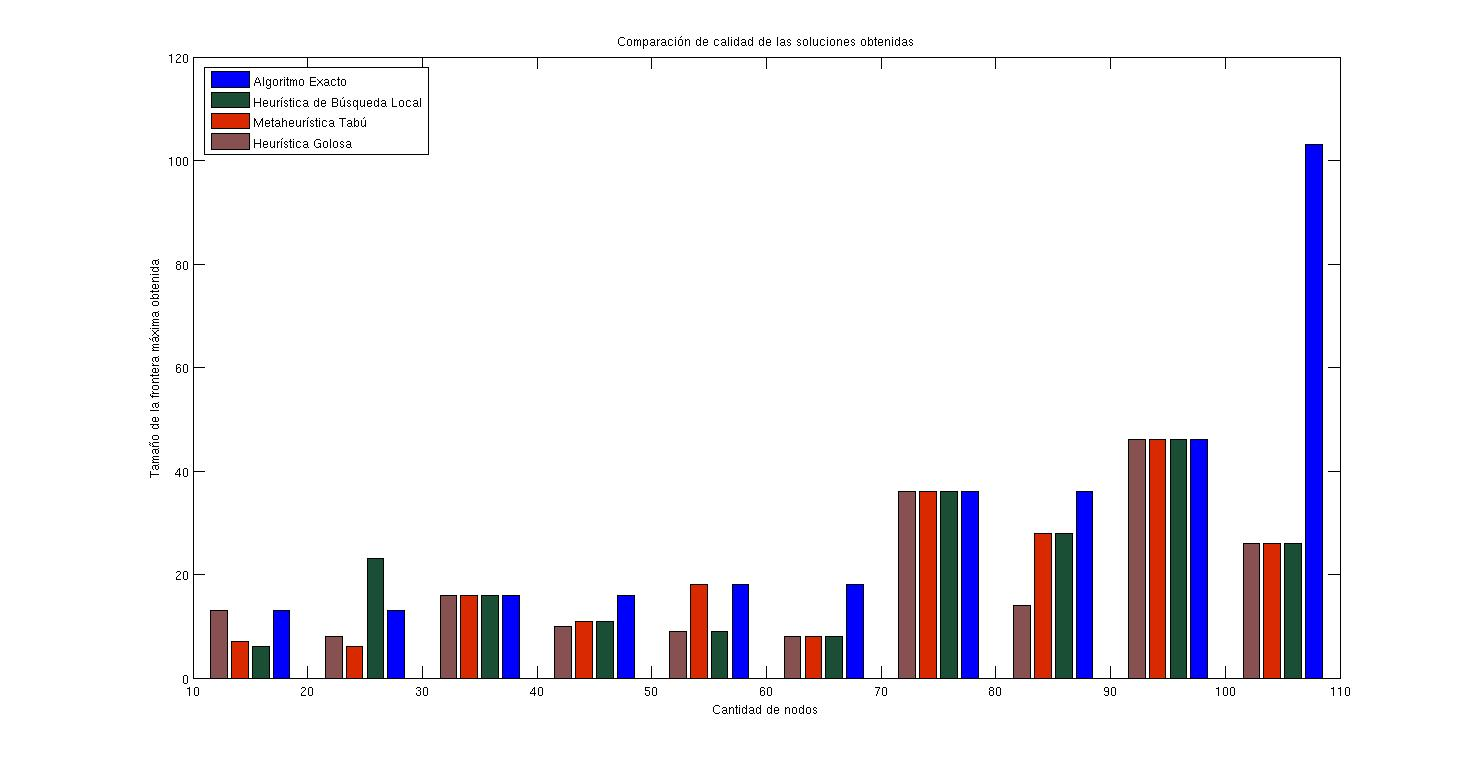
\includegraphics[width=400pt]{../imgs/calidadSolucionesChicas3.jpg}
\caption{Comparación realizada con soluciones chicas con un grafo de tipo Banana Tree.}
\end{center}
\end{figure}

 \begin{figure}[H] %[h] Aqui [b] para button [t] para top
\begin{center}
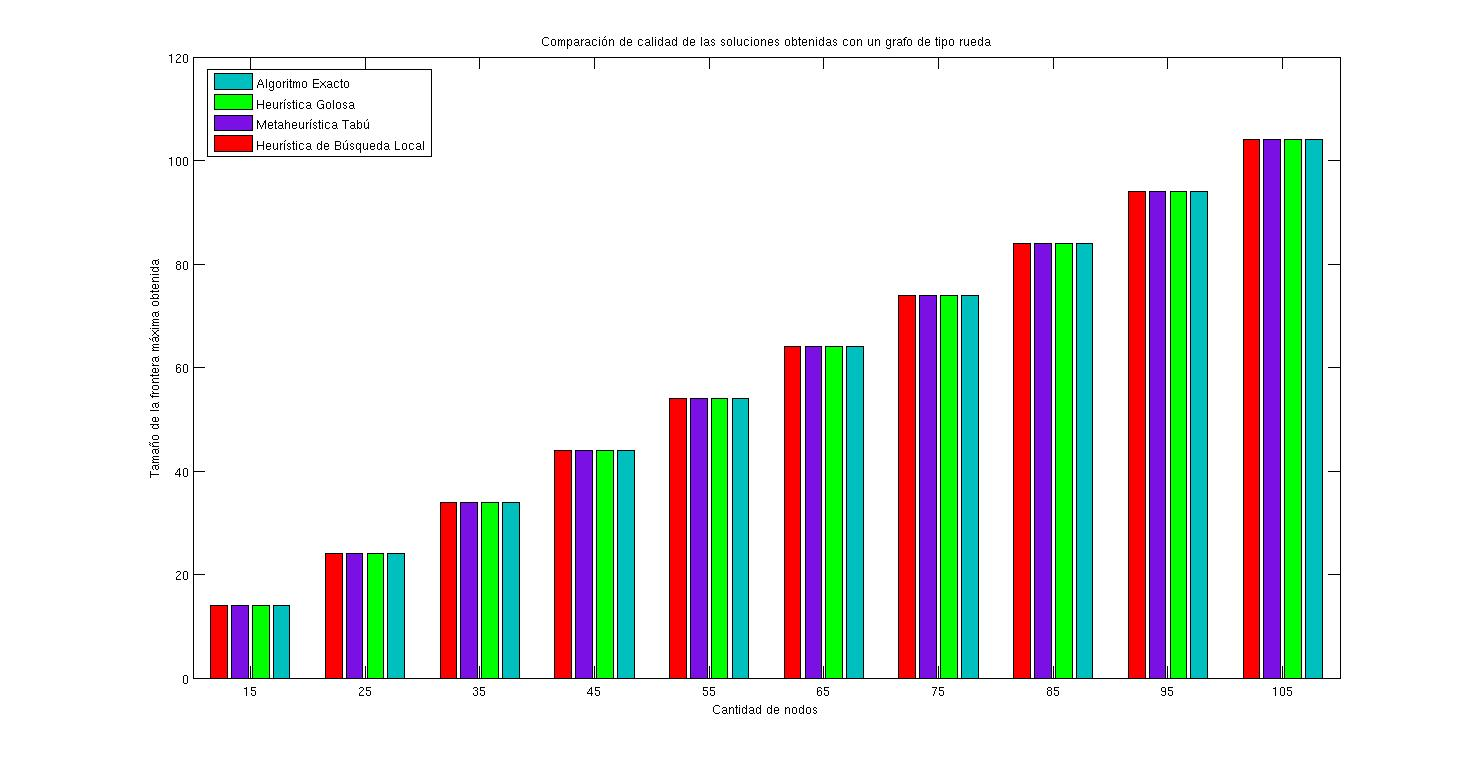
\includegraphics[width=400pt]{../imgs/calidadSolucionesChicas2.jpg}
\caption{Comparación realizada con soluciones chicas con un grafo de tipo rueda.}
\end{center}
\end{figure}

 \begin{figure}[H] %[h] Aqui [b] para button [t] para top
\begin{center}
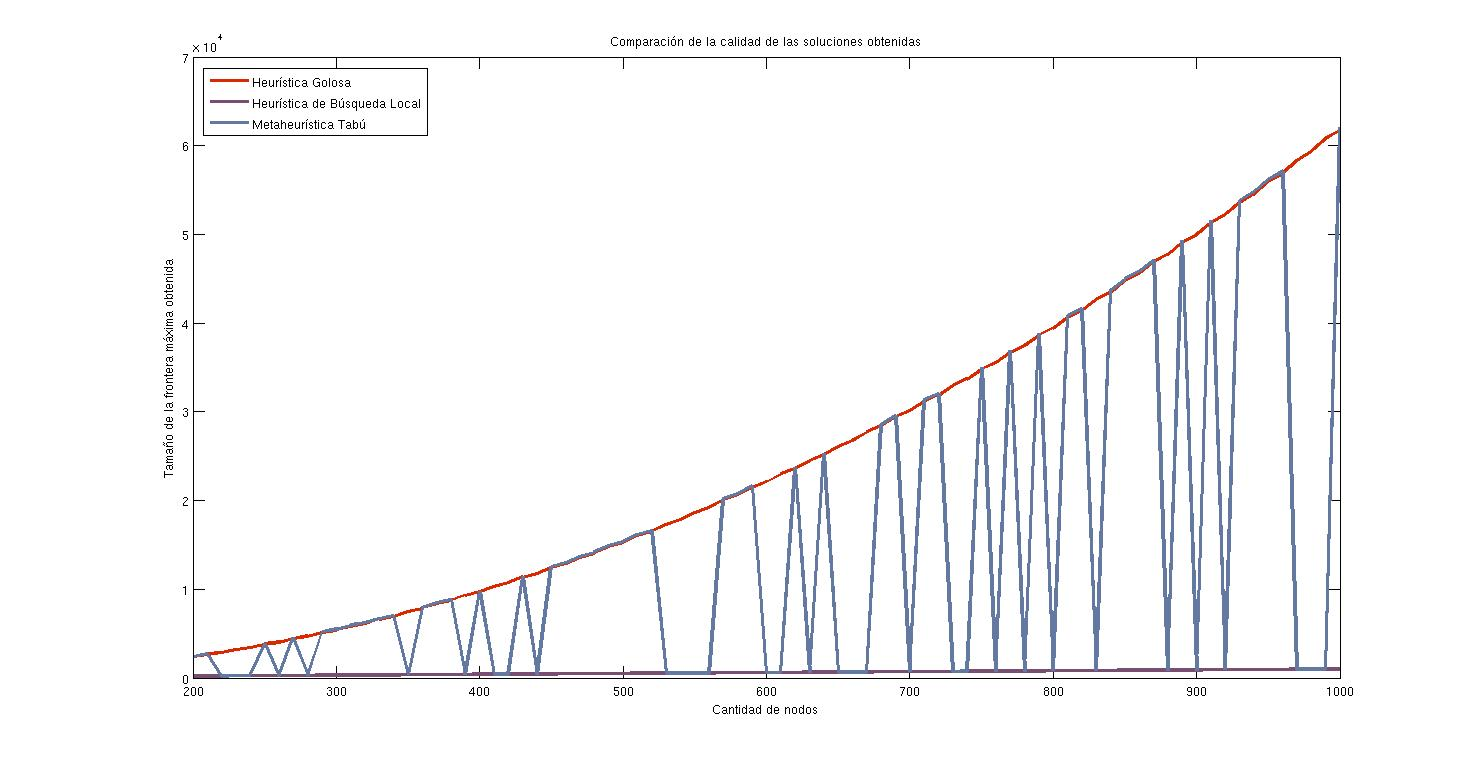
\includegraphics[width=400pt]{../imgs/calidadSolucionesGrandes15.jpg}
\caption{Comparación realizada con soluciones grandes con un grafo de tipo Estrella+CMF.}
\end{center}
\end{figure}

 \begin{figure}[H] %[h] Aqui [b] para button [t] para top
\begin{center}
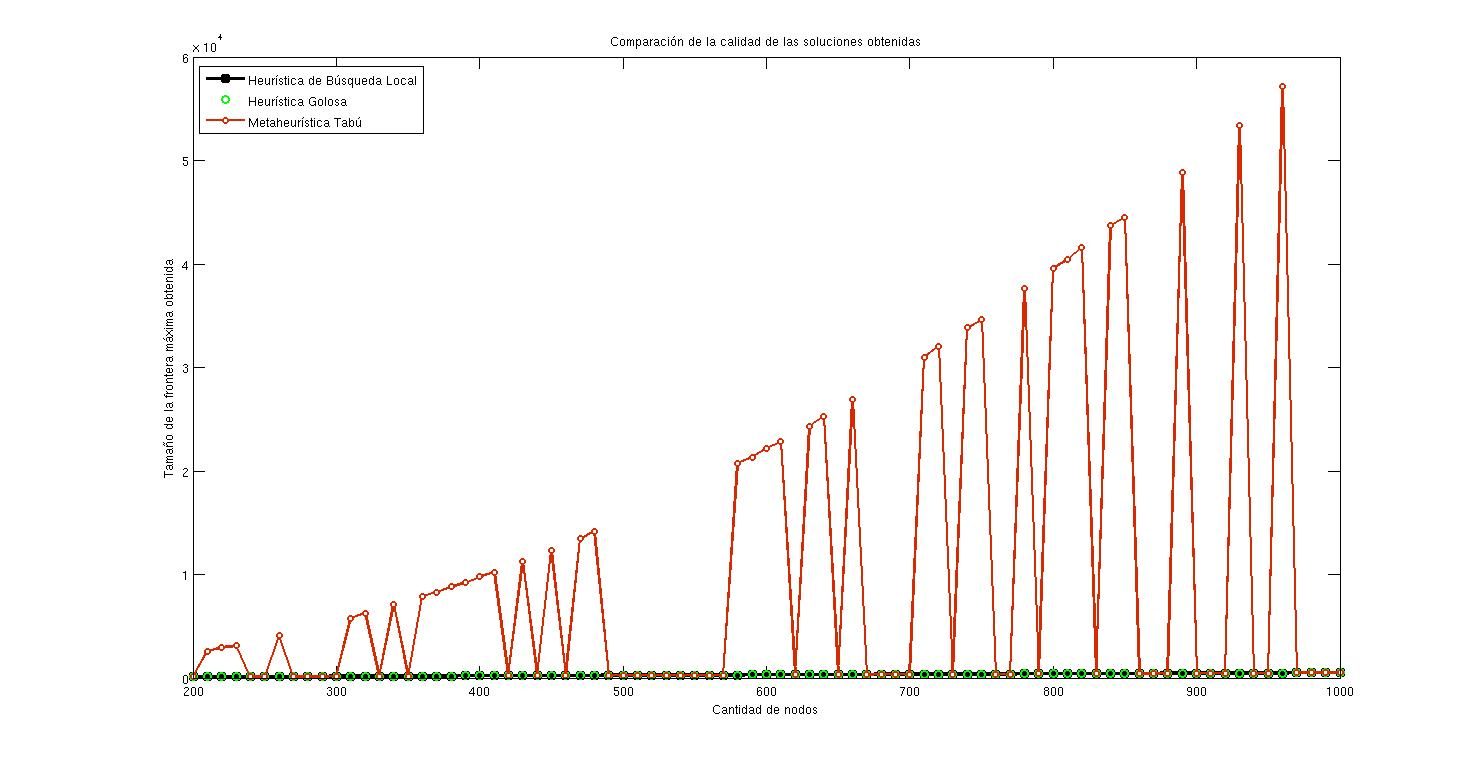
\includegraphics[width=400pt]{../imgs/calidadSolucionesGrandes14.jpg}
\caption{Comparación realizada con soluciones grandes con un grafo de tipo Estrella+Puente+CMF.}
\end{center}
\end{figure}

 \begin{figure}[H] %[h] Aqui [b] para button [t] para top
\begin{center}
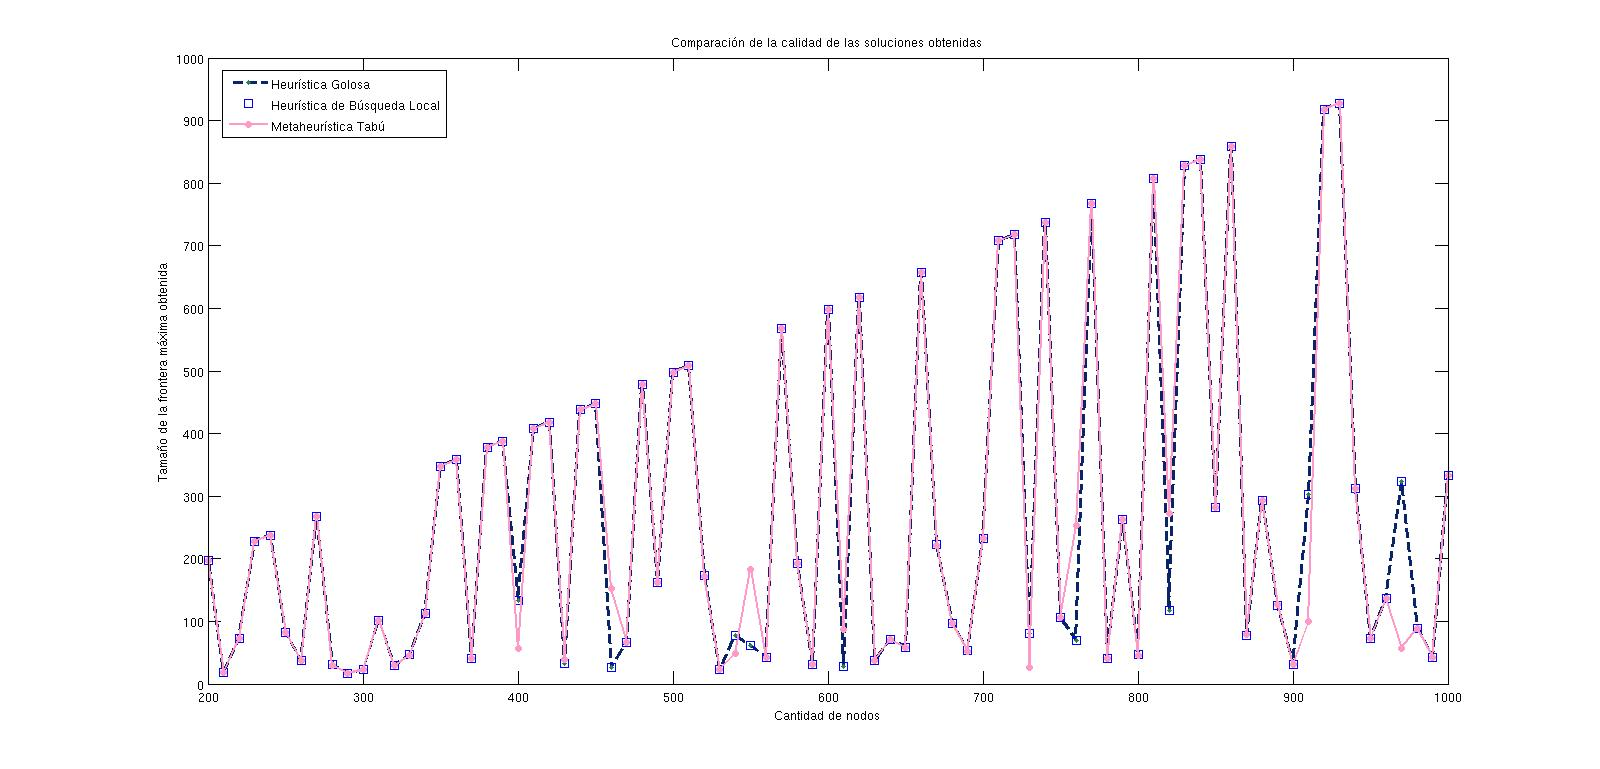
\includegraphics[width=400pt]{../imgs/calidadSolucionesGrandes3.jpg}
\caption{Comparación realizada con soluciones grandes con un grafo de tipo Banana Tree.}
\end{center}
\end{figure}
